% this file is called up by thesis.tex
% content in this file will be fed into the main document

%: ----------------------- introduction file header -----------------------
\chapter{Introduction}

% the code below specifies where the figures are stored
\ifpdf
    \graphicspath{{1_introduction/figures/PNG/}{1_introduction/figures/PDF/}{1_introduction/figures/}}
\else
    \graphicspath{{1_introduction/figures/EPS/}{1_introduction/figures/}}
\fi

This is how you cite~\citep{Moore99}.

Single sample image. 
\begin{figure}[!htbp]
\centering
\centering
   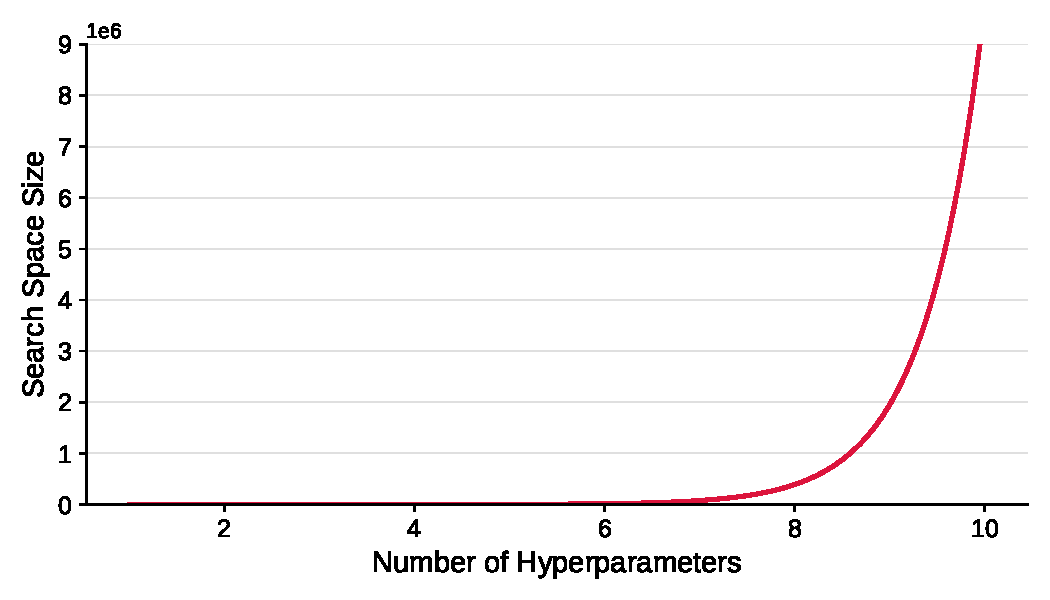
\includegraphics[width=0.8\textwidth]{1_introduction/figures/search_space.pdf}
   \caption{}
   \label{fig:abc}
\end{figure}


Sample subfigures.
\begin{figure}[!htbp]
\centering
\begin{subfigure}[b]{\textwidth}
\centering
   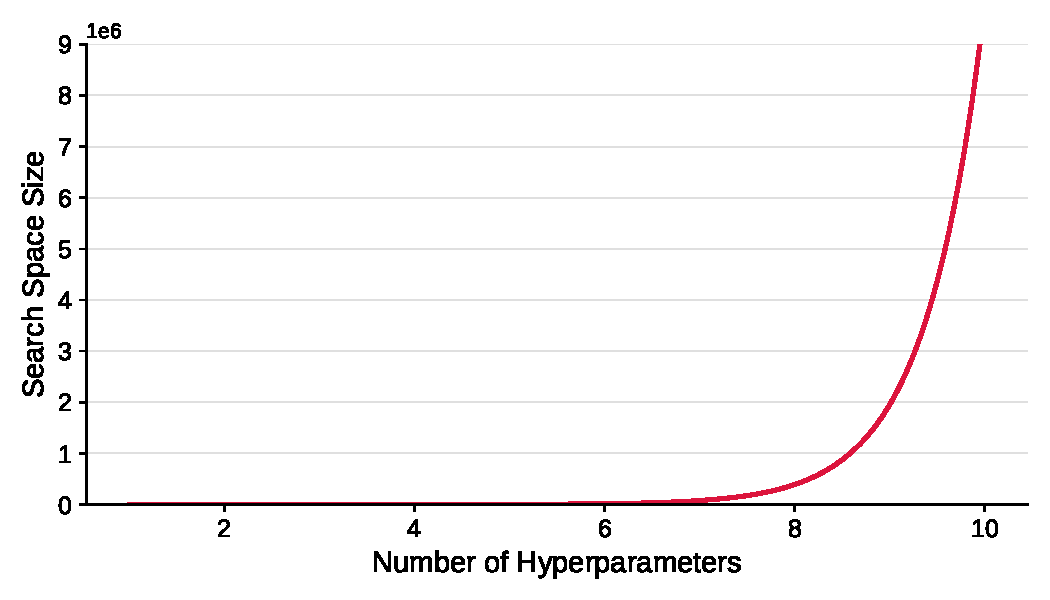
\includegraphics[width=0.4\textwidth]{1_introduction/figures/search_space.pdf}
   \caption{}
   \label{fig:search_space_exp}
\end{subfigure}
\begin{subfigure}[b]{\textwidth}
\centering
   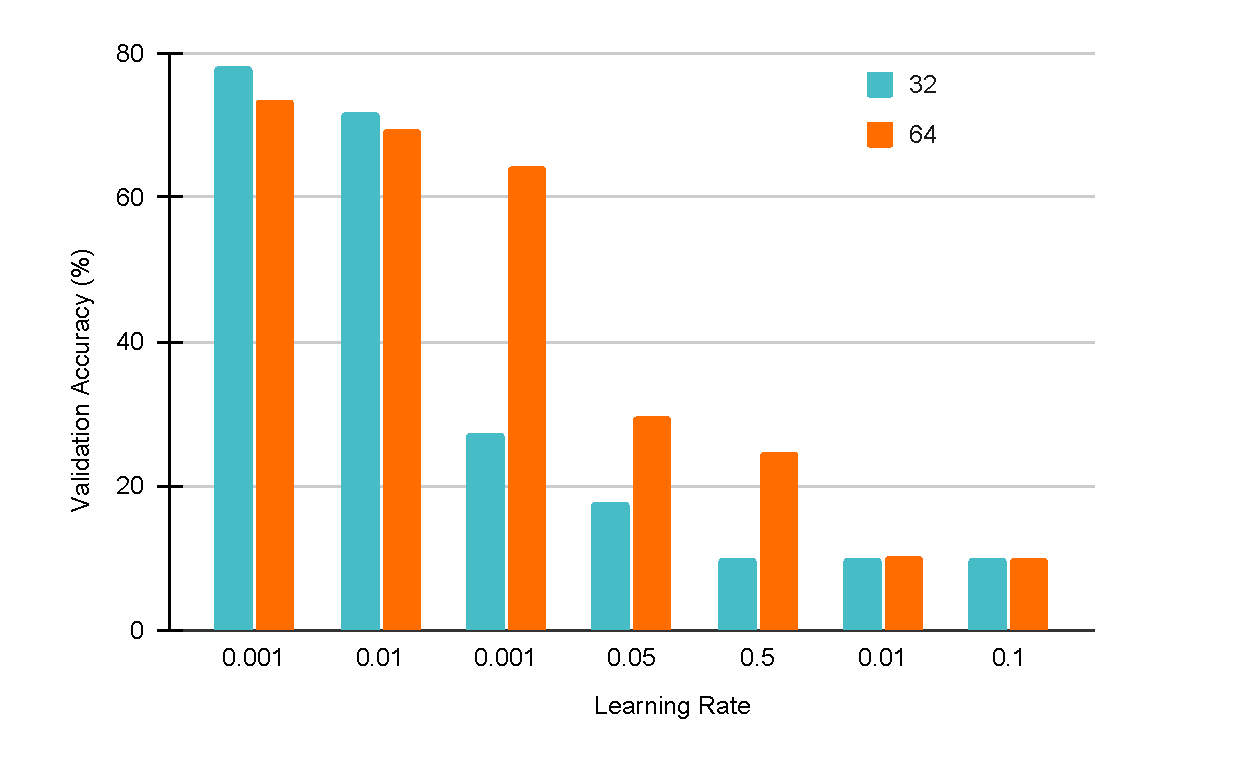
\includegraphics[width=0.4\textwidth]{1_introduction/figures/impact-of-hyp.pdf}
   \caption{}
   \label{fig:impact_hyper}
\end{subfigure}
\begin{subfigure}[c]{\textwidth}
\centering
   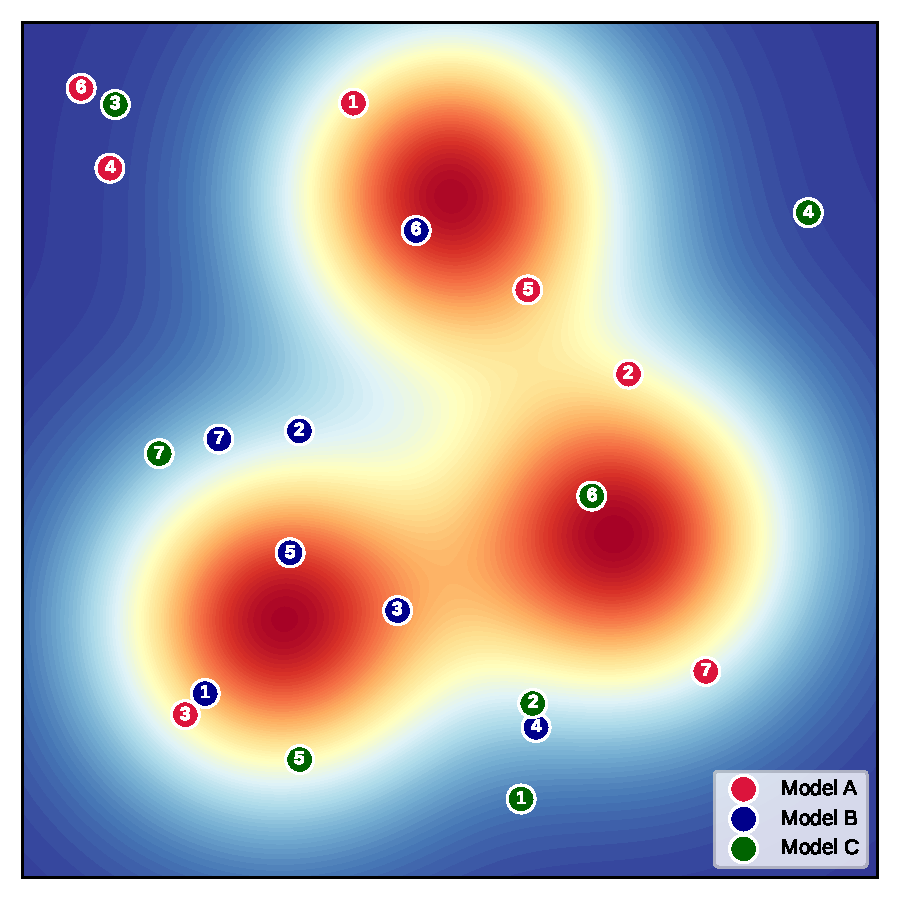
\includegraphics[width=0.4\textwidth]{1_introduction/figures/fitness_landscape.pdf}
   \caption{}
   \label{fig:fitness_landscape}
\end{subfigure}
\caption{Sample.
(a) Caption 1;
(b) Caption 2;
(c) Caption 3.}
\label{fig:challenges}
\end{figure}



% ------------------- Table Start -------------------
\begin{table}[!htb]
\caption{Sample hyperparameter configurations.}
\center
\begin{tabular}{lccc}
\hlineB{2}
\textbf{Optimizer} & \textbf{Learning Rate} & \textbf{Batch Size} & \textbf{Validation Accuracy} \\ \hlineB{2}
adam & \(1.00 \times 10^{-3}\) & 128 & 0.14 \\
adam & \(1.00 \times 10^{-4}\) & 128 & 0.57 \\
rmsprop & \(1.00 \times 10^{-4}\) & 32 & 0.52 \\
rmsprop & \(1.00 \times 10^{-3}\) & 16 & 0.14 \\
rmsprop & \(1.00 \times 10^{-6}\) & 8 & 0.43 \\ \hlineB{2}
\end{tabular}
\label{tab:sample_individuals}
\end{table}
% ------------------- Table End -------------------

